\chapter{
طراحی
مدار چاپی
یا
PCB
}

\section{
تغییرات مورد نیاز در بخش شماتیک
}
با این که هدف ما در این جلسه تنها طراحی همان شماتیک روی مدار چاپی است، اما باید تغییرات کوچکی در قسمت شماتیک نیز ایجاد کنیم تا بتوانیم مدار را به راحتی و بدون خطا در قسمت طراحی مدار چاپی پیاده کنیم.

\subsection{
ایجاد کانکتور برای ورودی‌ها و خروجی‌های مدار
}
در قسمت شماتیک از قطعات مخصوص دیباگ برای تعیین ورودی‌ها و مشاهده‌ی خروجی‌ها استفاده می‌کردیم.
اما برای طراحی مدار چاپی بهتر است در قسمت شماتیک قطعات کانکتور را هم به صورت موازی قرار دهیم.

قطعات دیباگ در قسمت چاپی نادیده گرفته خواهند شد. (در صورتی که تنظیمات پیش‌فرض این نبود می‌توان در پنجره‌ی تنظیمات هر قطعه تیک
\lr{Exclude from PCB Layout}
آن را فعال کرد)

\subsection{
جایگزین قطعات بدون مدل چاپی
}
برخی از قطعات شماتیک مدل فیزیکی ندارند
در مدار ما گیت‌های استفاده شده گیت‌های مدل پروتئوس هستند و شماتیک یک
IC
فیزیکی نیستند.
باید این قطعات را با جایگزین
مثلا
74xx
خود تعویض کرد.

البته باید دقت کنیم نمی‌توان به سادگی آن‌ها را روی قطعه‌ی قبلی قرار داد چرا که متاسفانه پروتئوس برای جایگزین کردن دو قطعه هر بار از یک
IC
جدید استفاده می‌کند و مثلا گیت اند را همیشه به اولین گیت اند
IC
مقصد مپ می‌کند.
اما ما می‌خواهیم از هر ۴ گیتی که به طور معمول در یک
IC
وجود دارد استفاده کنیم.
برای این کار چاره‌ای جز حذف قبلی‌ها و افزودن دستی جدیدها نداریم.

\subsection{
تغییر مدل چاپی برخی قطعات
}
برخی قطعات مدل‌های چاپی متعددی دارند. در صورتی که برای قطعه‌ای که مدل چاپی داشت با خطایی در قسمت چاپی مواجه شدیم،
(که پیدا کردن قطعات دارای مشکل از لاگ خطاها قابل انجام است.)
کافی است با رفتن به
Properties
آن، مدل چاپی آن را تغییر دهیم.
در تصویر
\eqref{fig:prot1}
نمونه‌ای از این کار آمده.

\begin{figure}[h!]
    \centering
    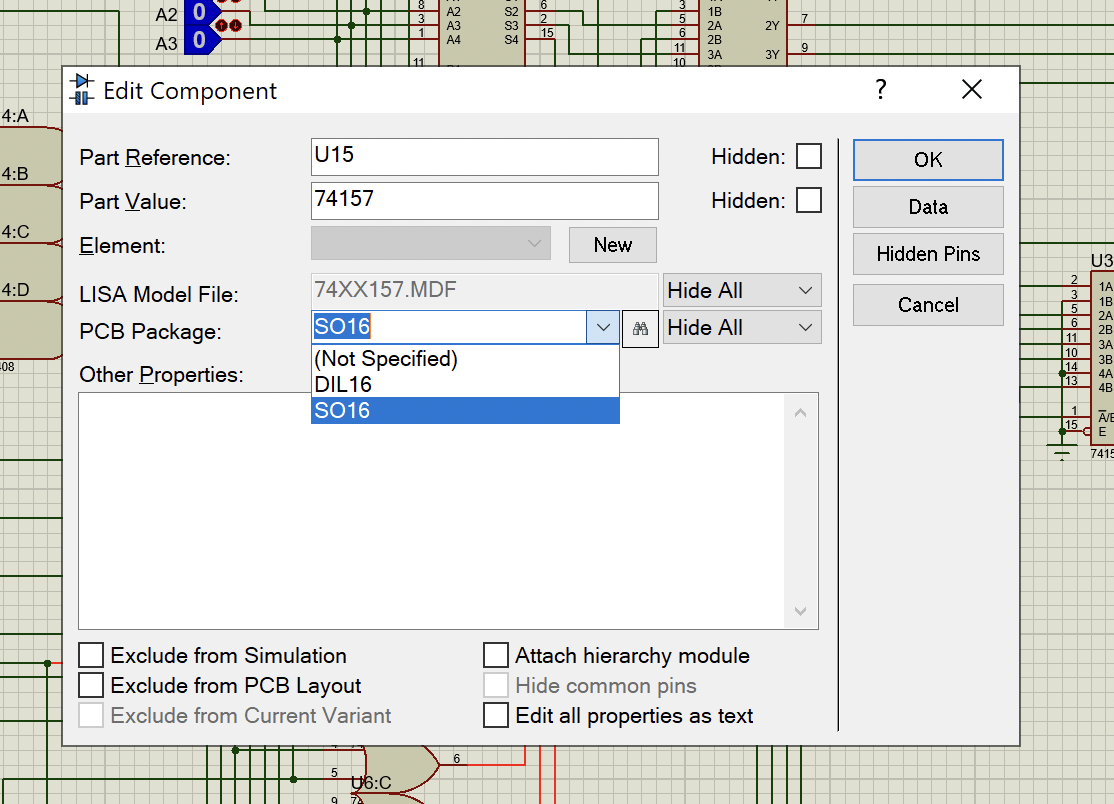
\includegraphics[width=0.6\textwidth]{images/ALU-PCB-Model.png}
    \caption{
    تغییر مدل چاپی
    }
    \label{fig:prot1}
\end{figure}

\paragraph{}
با انجام این کارها مدار برای طراحی چاپی آماده شده و باید بتوانیم قسمت طراحی چاپی نرم‌افزار را بدون
مشاهده‌ی هیچ خطایی در قسمت لاگ خطاها باز کنیم.
تصویر مدار نهایی اصلاح شده در
\eqref{fig:circuit1}
آمده است.

\begin{figure}[h!]
    \centering
    \includegraphics[width=\textwidth]{images/ALU-PCB.png}
    \caption{
    مدار شماتیک اصلاح شده
    }
    \label{fig:circuit1}
\end{figure}

\newpage

\section{
طراحی
}
پس از رفع خطاها در بخش قبل حال با موفقیت وارد بخش طراحی مدار چاپی نرم‌افزار می‌شویم.

در ابتدای کار با ابزار زرد نوار سمت چپ مرز مدار را مشخص می‌کنیم. سپس می‌توانیم با ابزارهای نوار بالایی زمینه‌ی مدار چاپی را برای تغذیه‌ی قطعات پر کنیم.
نرم‌افزار به طور خودکار وقتی نیاز باشد قسمتی از سمتی که برای تغذیه پر شده را خالی می‌کند و برای سیم‌کشی جدا می‌کند.

در نوار بالا دو گزینه‌ی
\lr{Auto-placer}
و
\lr{Auto-wire}
وجود دارند که عملیات‌های قرار دادن قطعات و 
سیم‌کشی بین آن‌ها را به طور خودکار بر اساس
تنظیماتی که در
\lr{Design Rule Manager}
\eqref{fig:rule}
انجام داده‌اید انجام می‌دهد.
تنظیمات پیش‌فرض نرم‌افزار برای کار ما مناسب هستند.

\begin{figure}[h!]
    \centering
    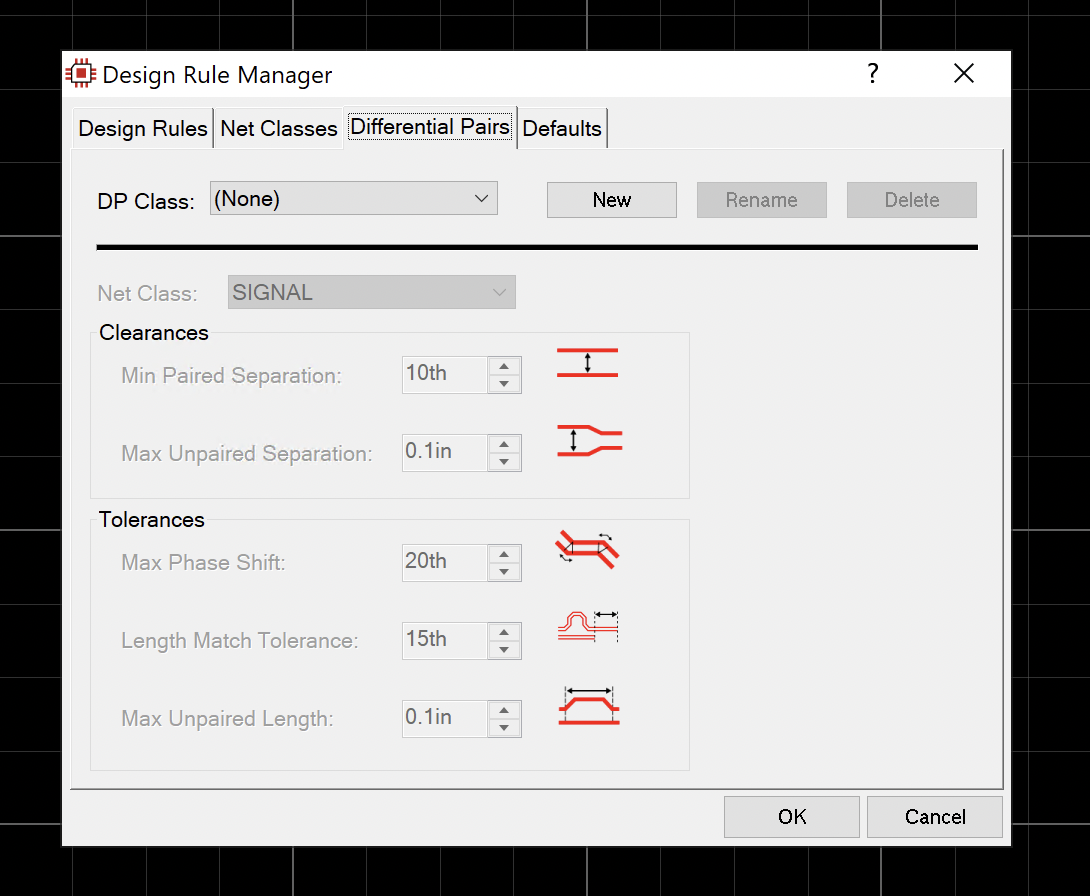
\includegraphics[width=0.7\textwidth]{images/ALU-PCB-Rule.png}
    \caption{
    قوانین عملیات‌های خودکار
    }
    \label{fig:rule}
\end{figure}

پس از این که از امکان قرارگیری خودکار استفاده کردیم، متوجه می‌شویم که خیلی جالب و مرتب قطعات را نمی‌چیند.
حال به صورت دستی قطعات را می‌چینیم. تا جای ممکن با توجه به اتصالاتی که نرم‌افزار نشان می‌دهد سعی می‌کنیم تا سیم‌کشی ما کمینه شود و از پیچیدگی آن کاسته شود.

در انتها پس از قرار گرفتن قطعات از امکان سیم‌کشی خودکار نرم‌افزار استفاده می‌کنیم.
\eqref{fig:wire}
تنظیمات پیش‌فرض نرم‌افزار مناسب هستند ولی در صورت داشتن سیستم‌قوی می‌توان کمی دفعات بررسی و پاک‌سازی را بیشتر کرد.

\begin{figure}[h!]
    \centering
    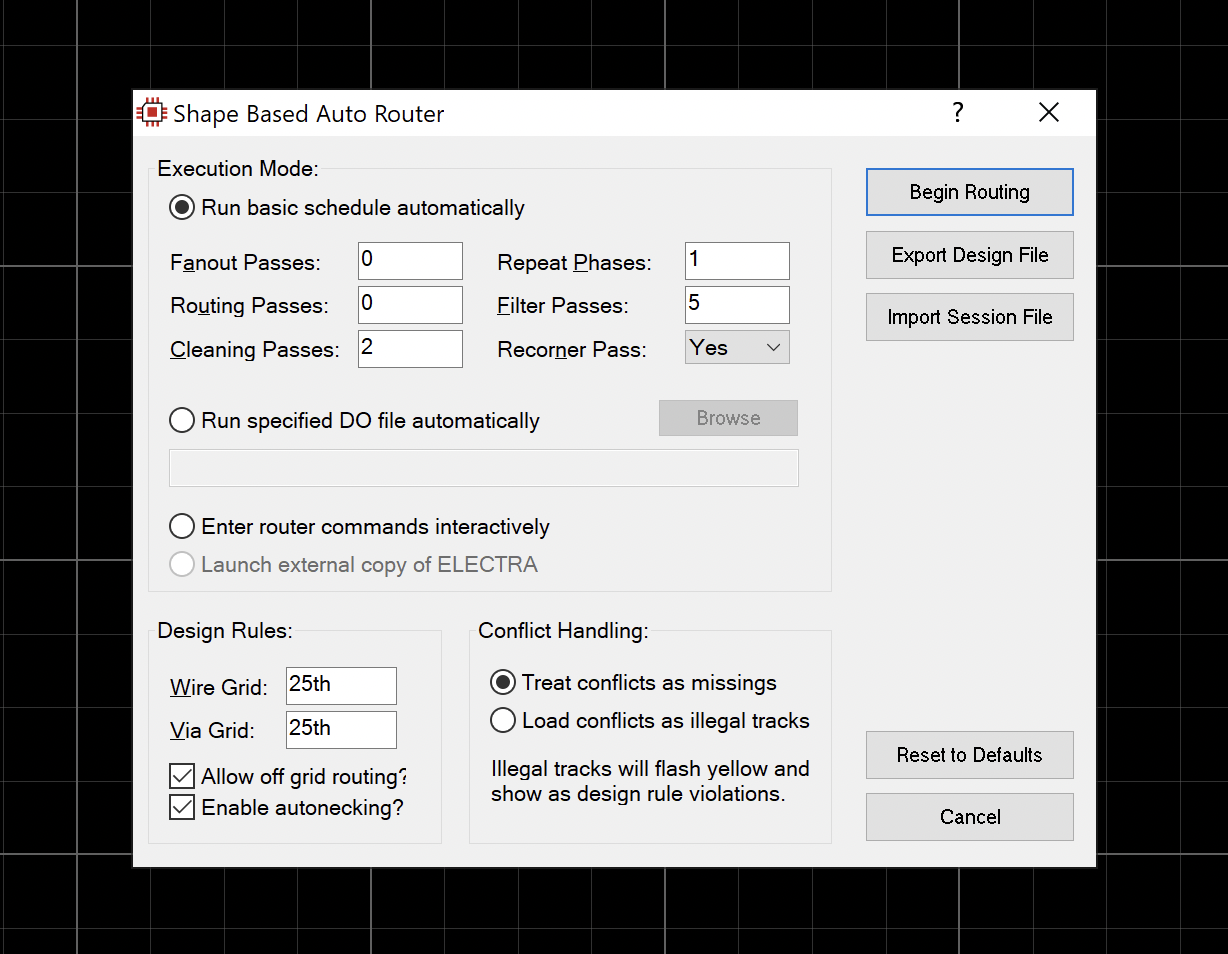
\includegraphics[width=\textwidth]{images/ALU-PCB-AutoConnection.png}
    \caption{
    تنظیمات سیم‌کشی خودکار
    }
    \label{fig:wire}
\end{figure}

در انتها مدار ما به شکل
\eqref{fig:final}
در خواهد آمد.

\begin{figure}[h!]
    \centering
    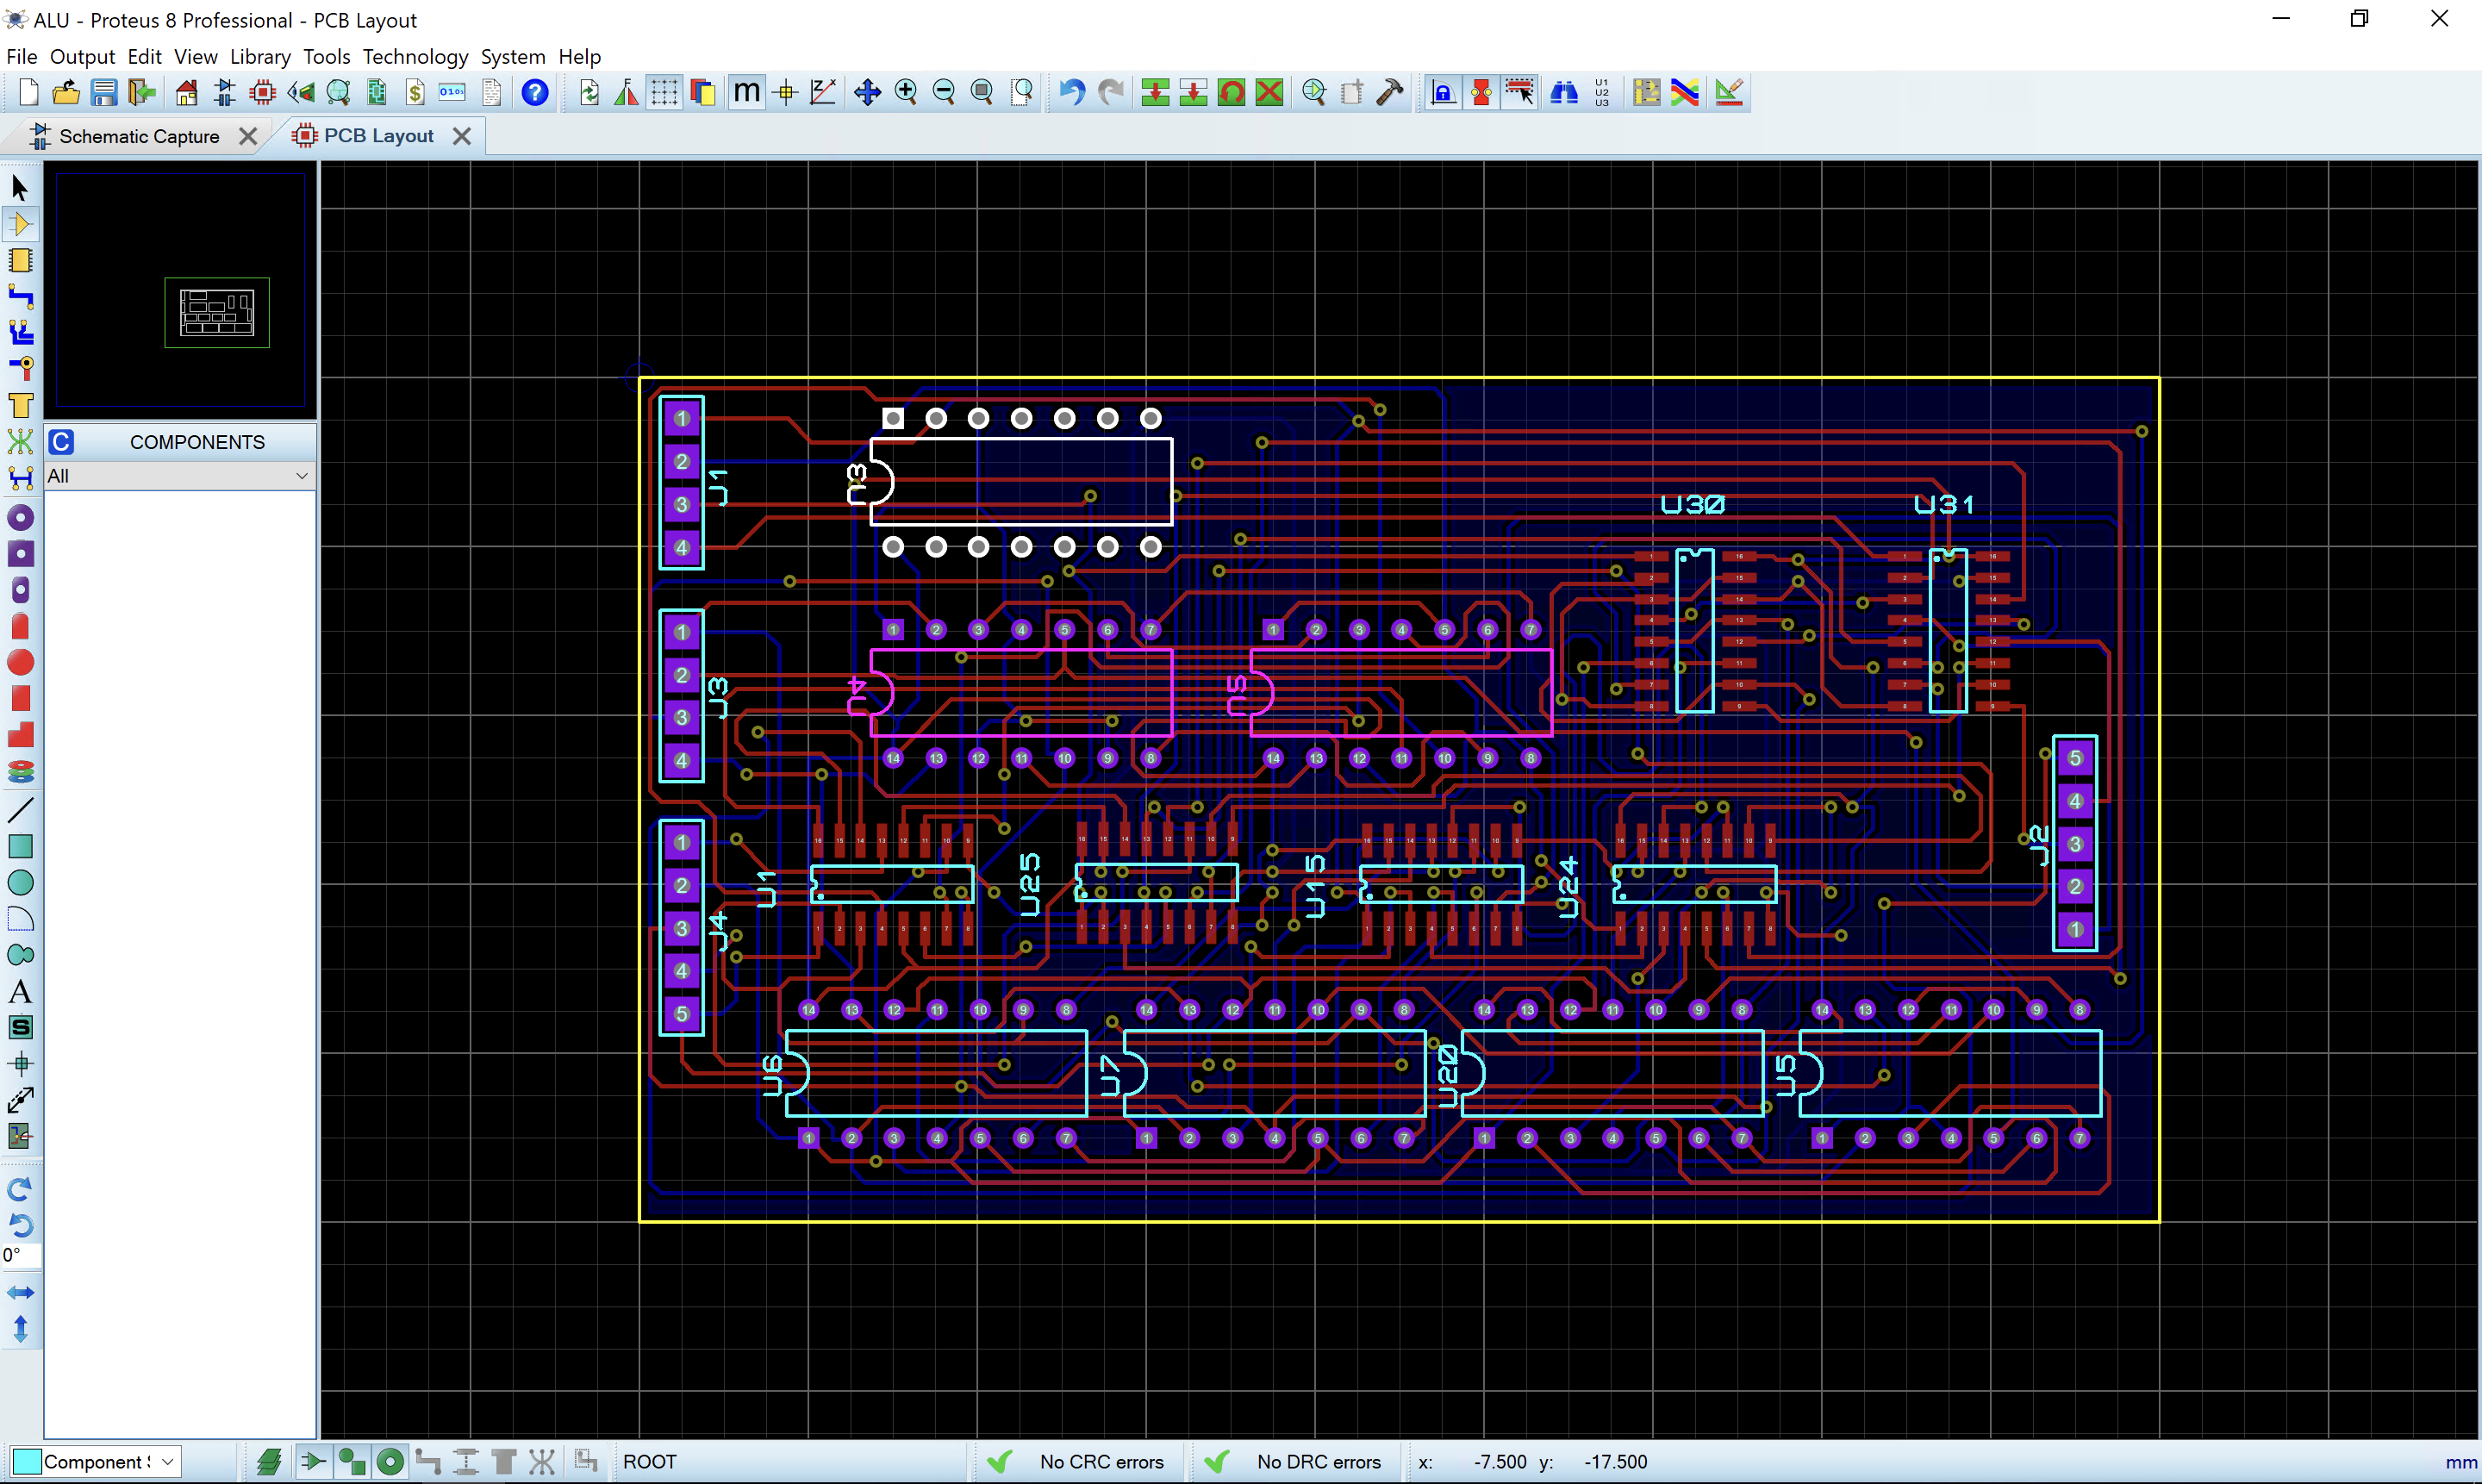
\includegraphics[width=\textwidth]{images/ALU-PCB-PR.png}
    \caption{
    مدار نهایی در محیط نرم‌افزار
    }
    \label{fig:final}
\end{figure}

\begin{figure}[h!]
    \centering
    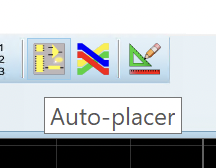
\includegraphics[width=0.3\textwidth]{images/ALU-PCB-AutoPlacer.png}
    \caption{
    عملیات‌های خودکار در نوار بالا
    }
\end{figure}

\section{
خروجی‌ها و رندر سه‌بعدی
}
نرم‌افزار پروتئوس امکان خروجی طراحی را با فرمت‌های متعددی در اختیار ما می‌گذارد. حتی می‌توانیم یک رندر سه‌بعدی از شکل برد چاپی را
ببینیم و با فرمت‌های معروف شکل سه‌بعدی خروجی بگیریم.

در اینجا به تصاویری از رندر سه‌بعدی و دو تصویر از شکل بالا و پایین برد چاپی اکتفا شده اما در فایل‌های ارسالی خروجی‌های سه‌بعدی نیز قرار داده شده‌اند.

\begin{figure}[h!]
    \centering
    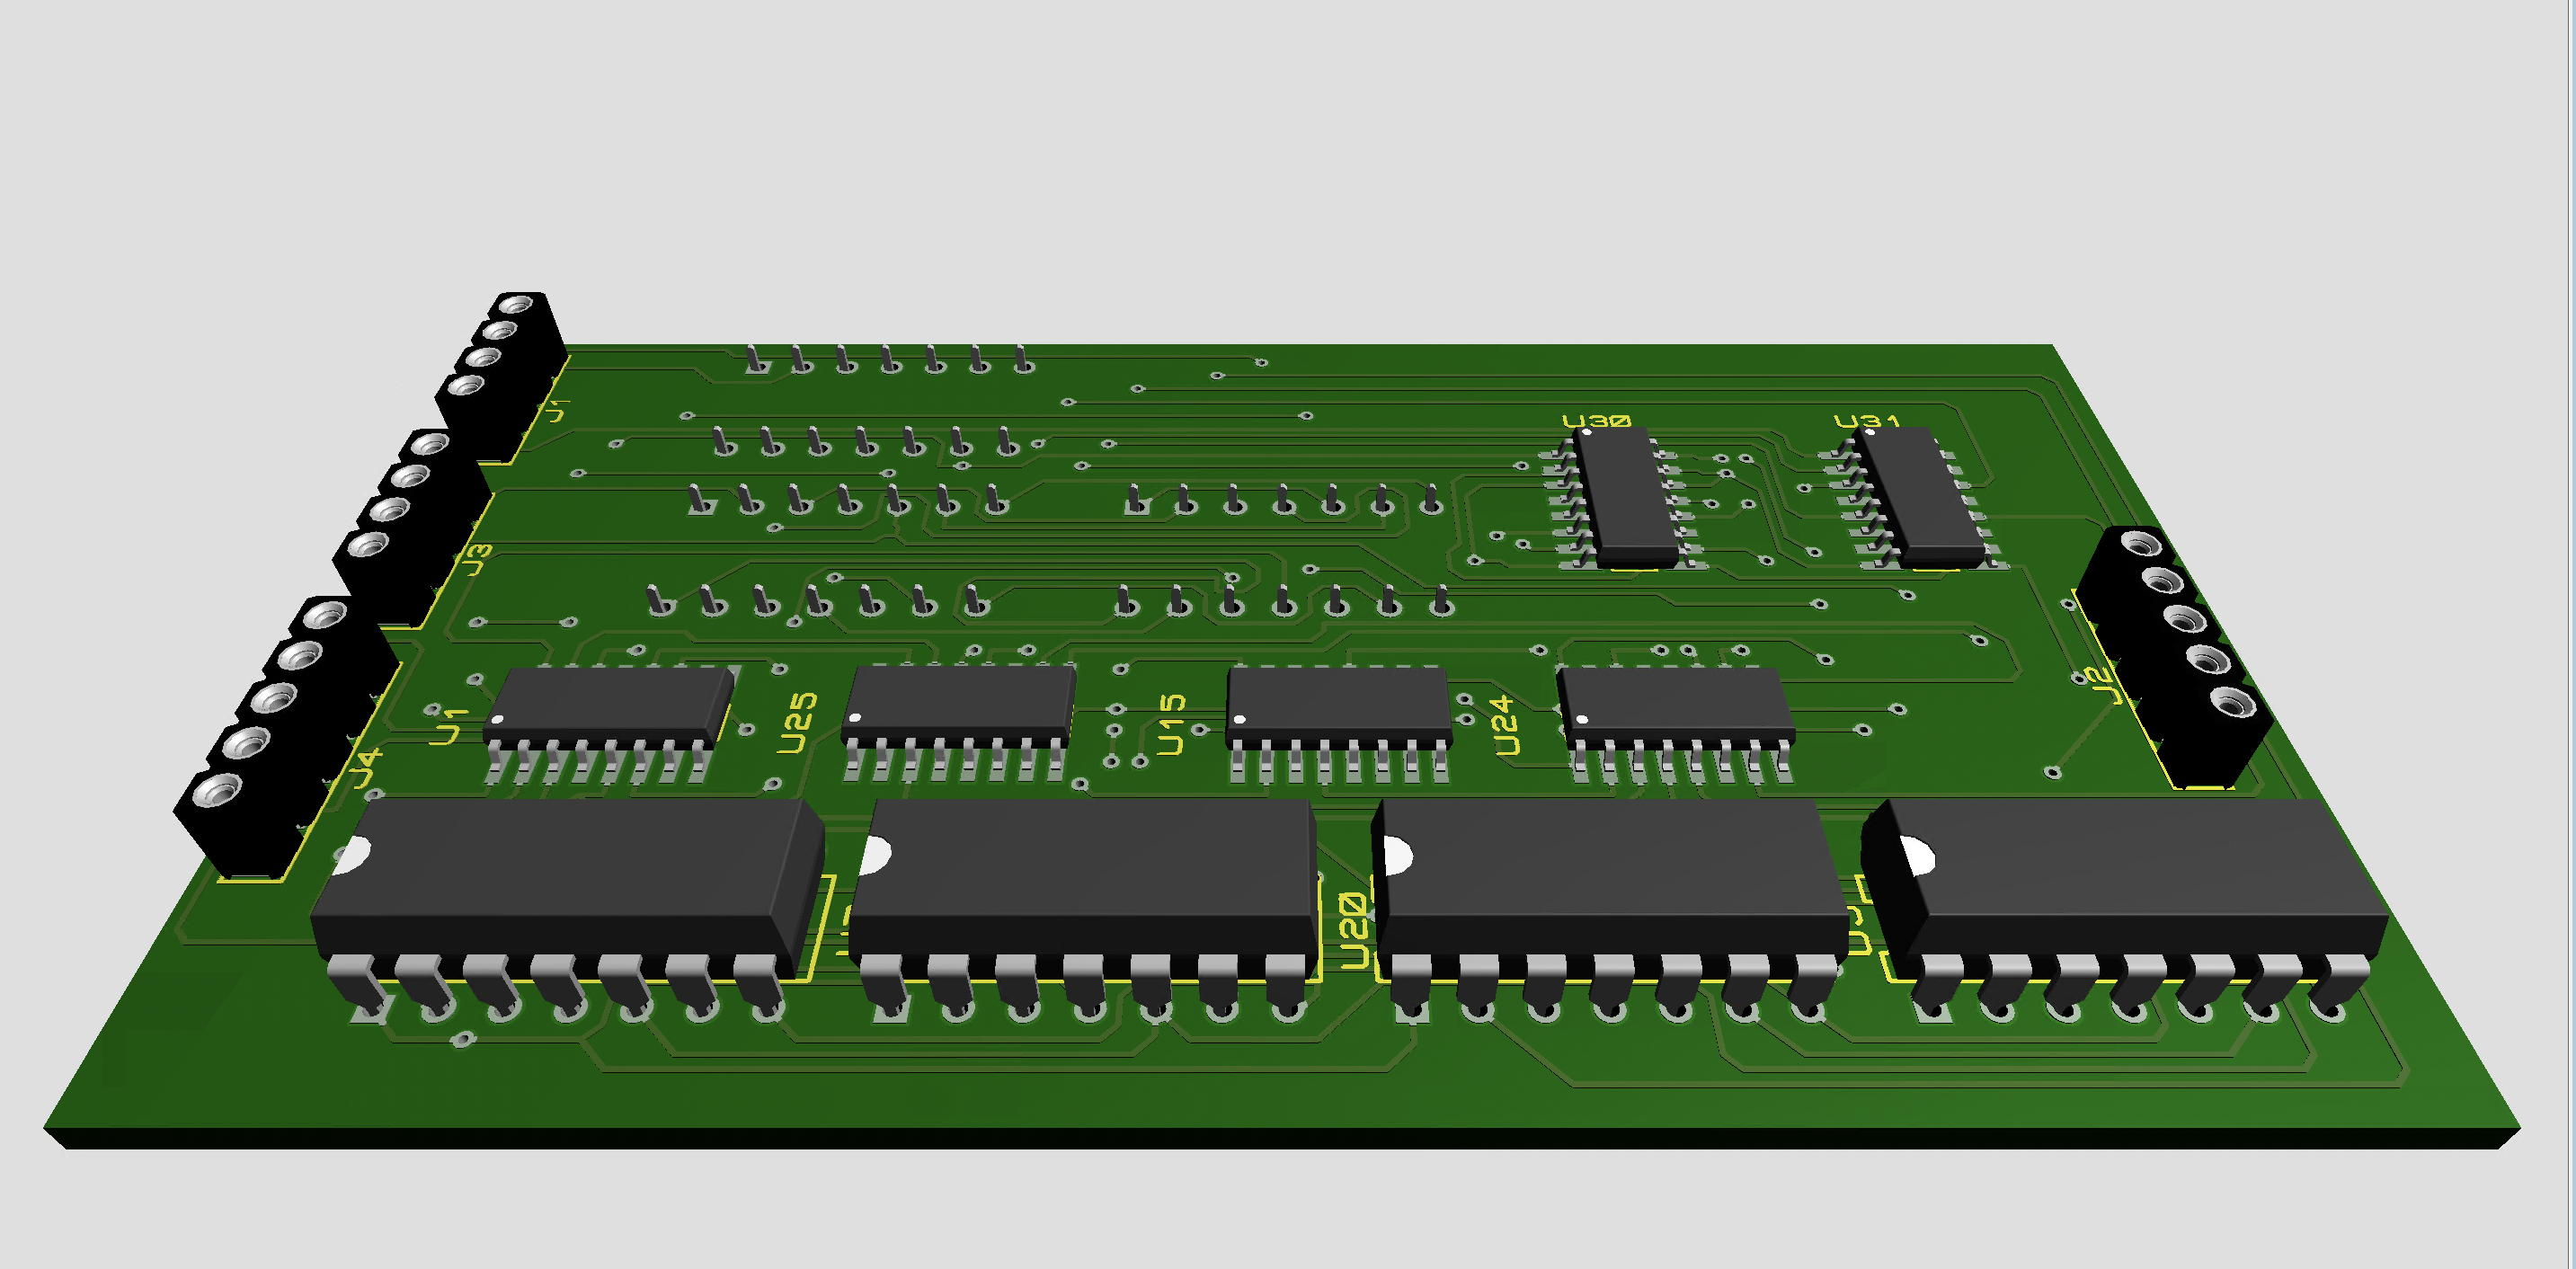
\includegraphics[width=\textwidth]{images/ALU-PCB-3D.png}
    \caption{
    رندر سه‌بعدی برد
    }
\end{figure}

\begin{figure}[h!]
    \centering
    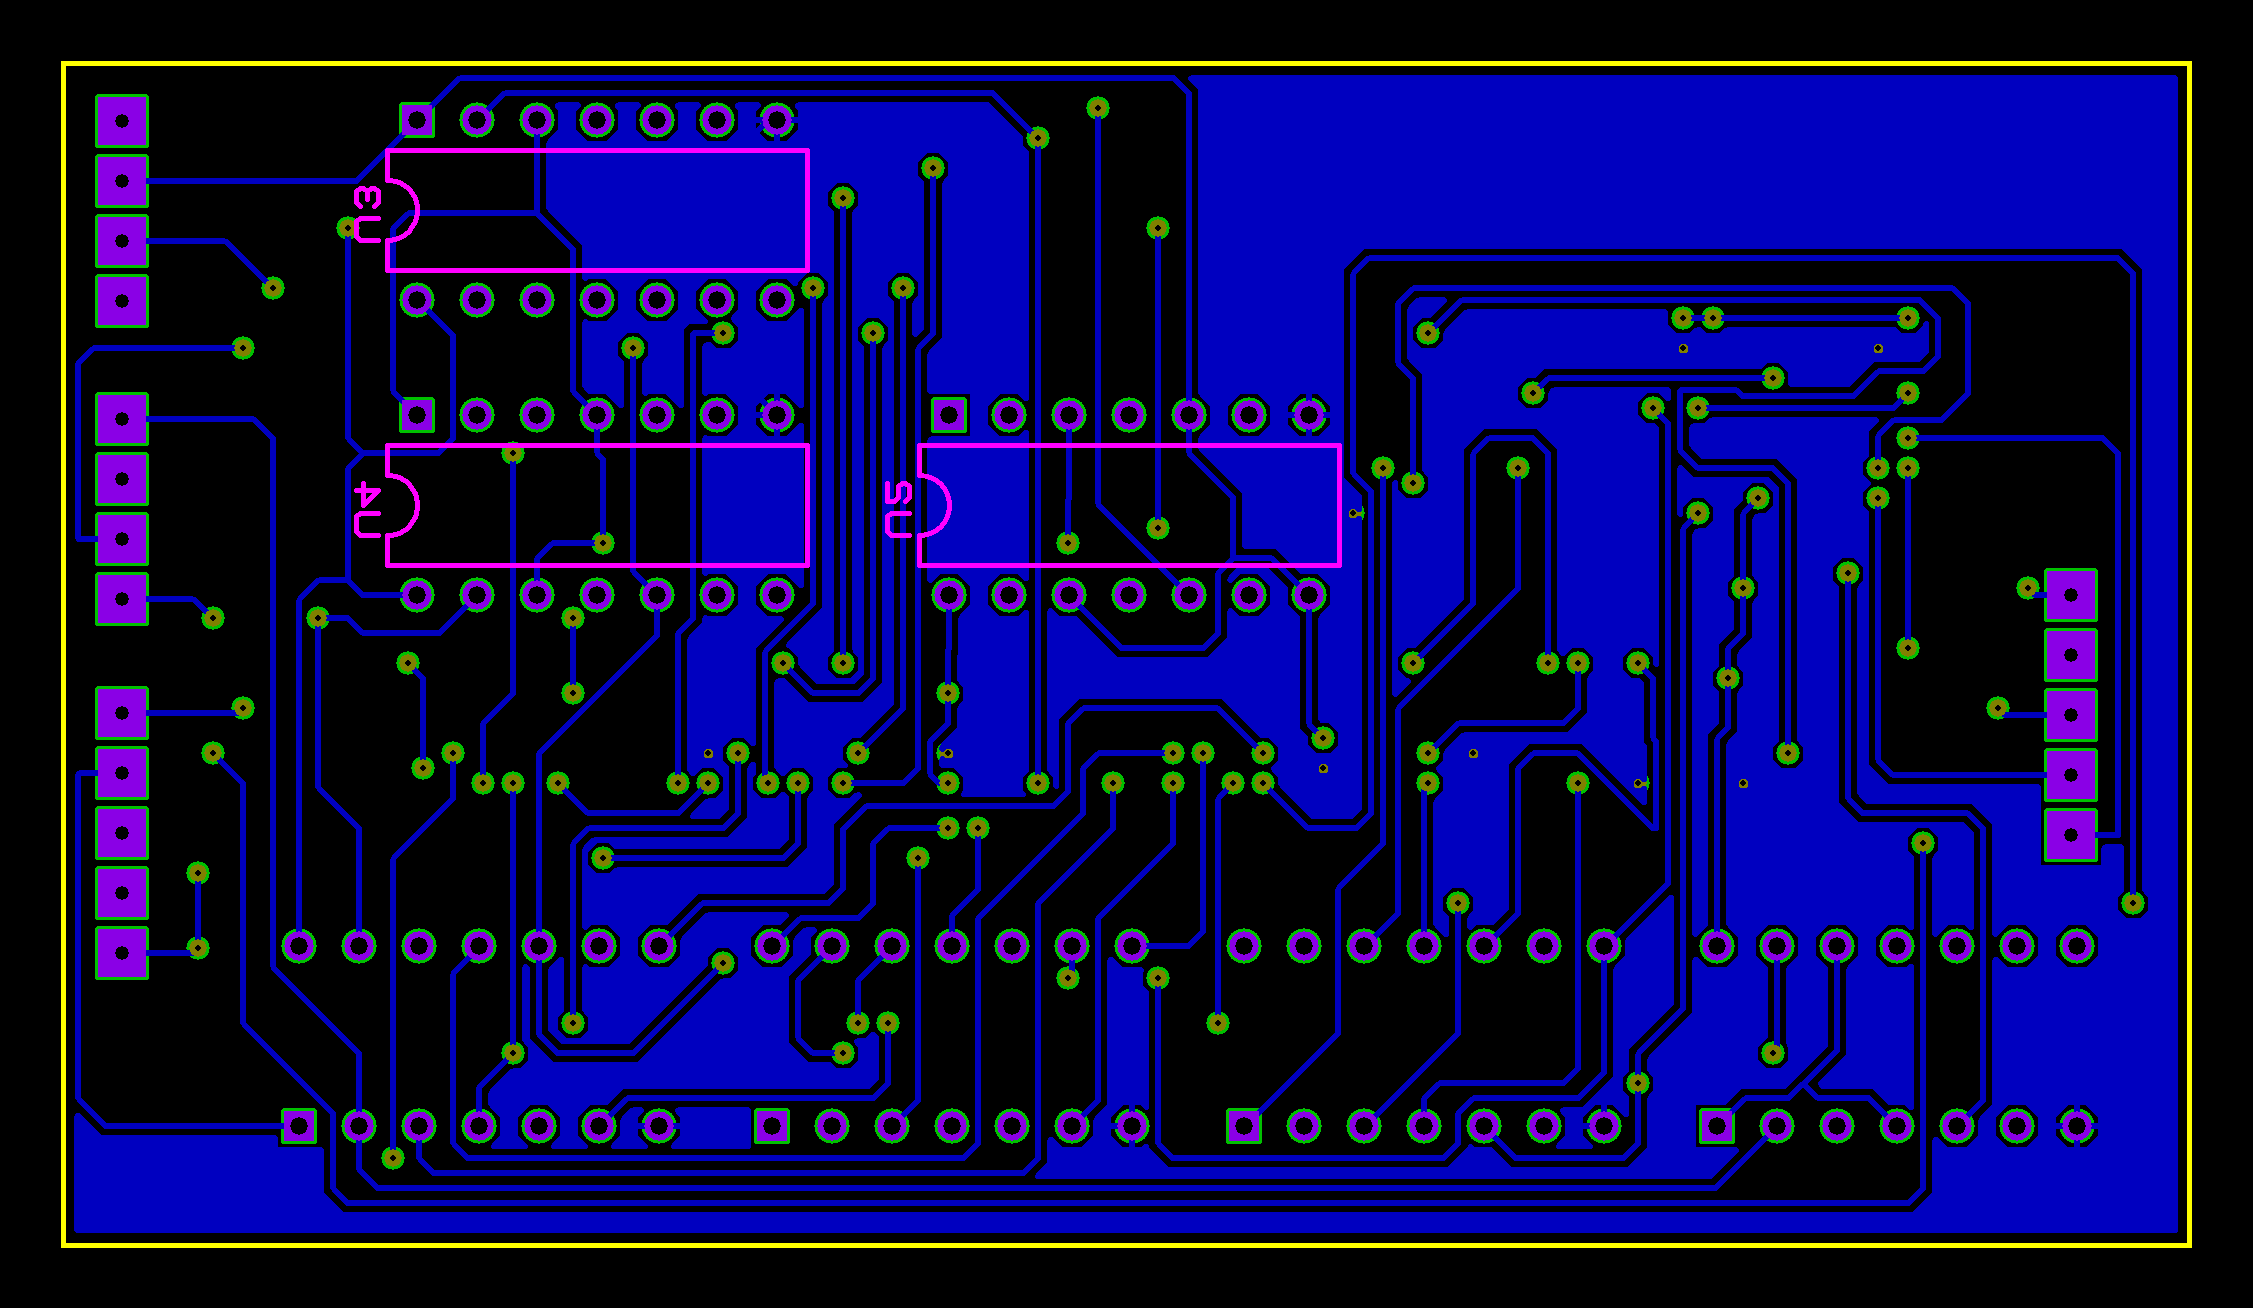
\includegraphics[width=\textwidth]{images/ALU-PCB-BOT.png}
    \caption{
    نمای زیر برد چاپی
    }
\end{figure}

\begin{figure}[h!]
    \centering
    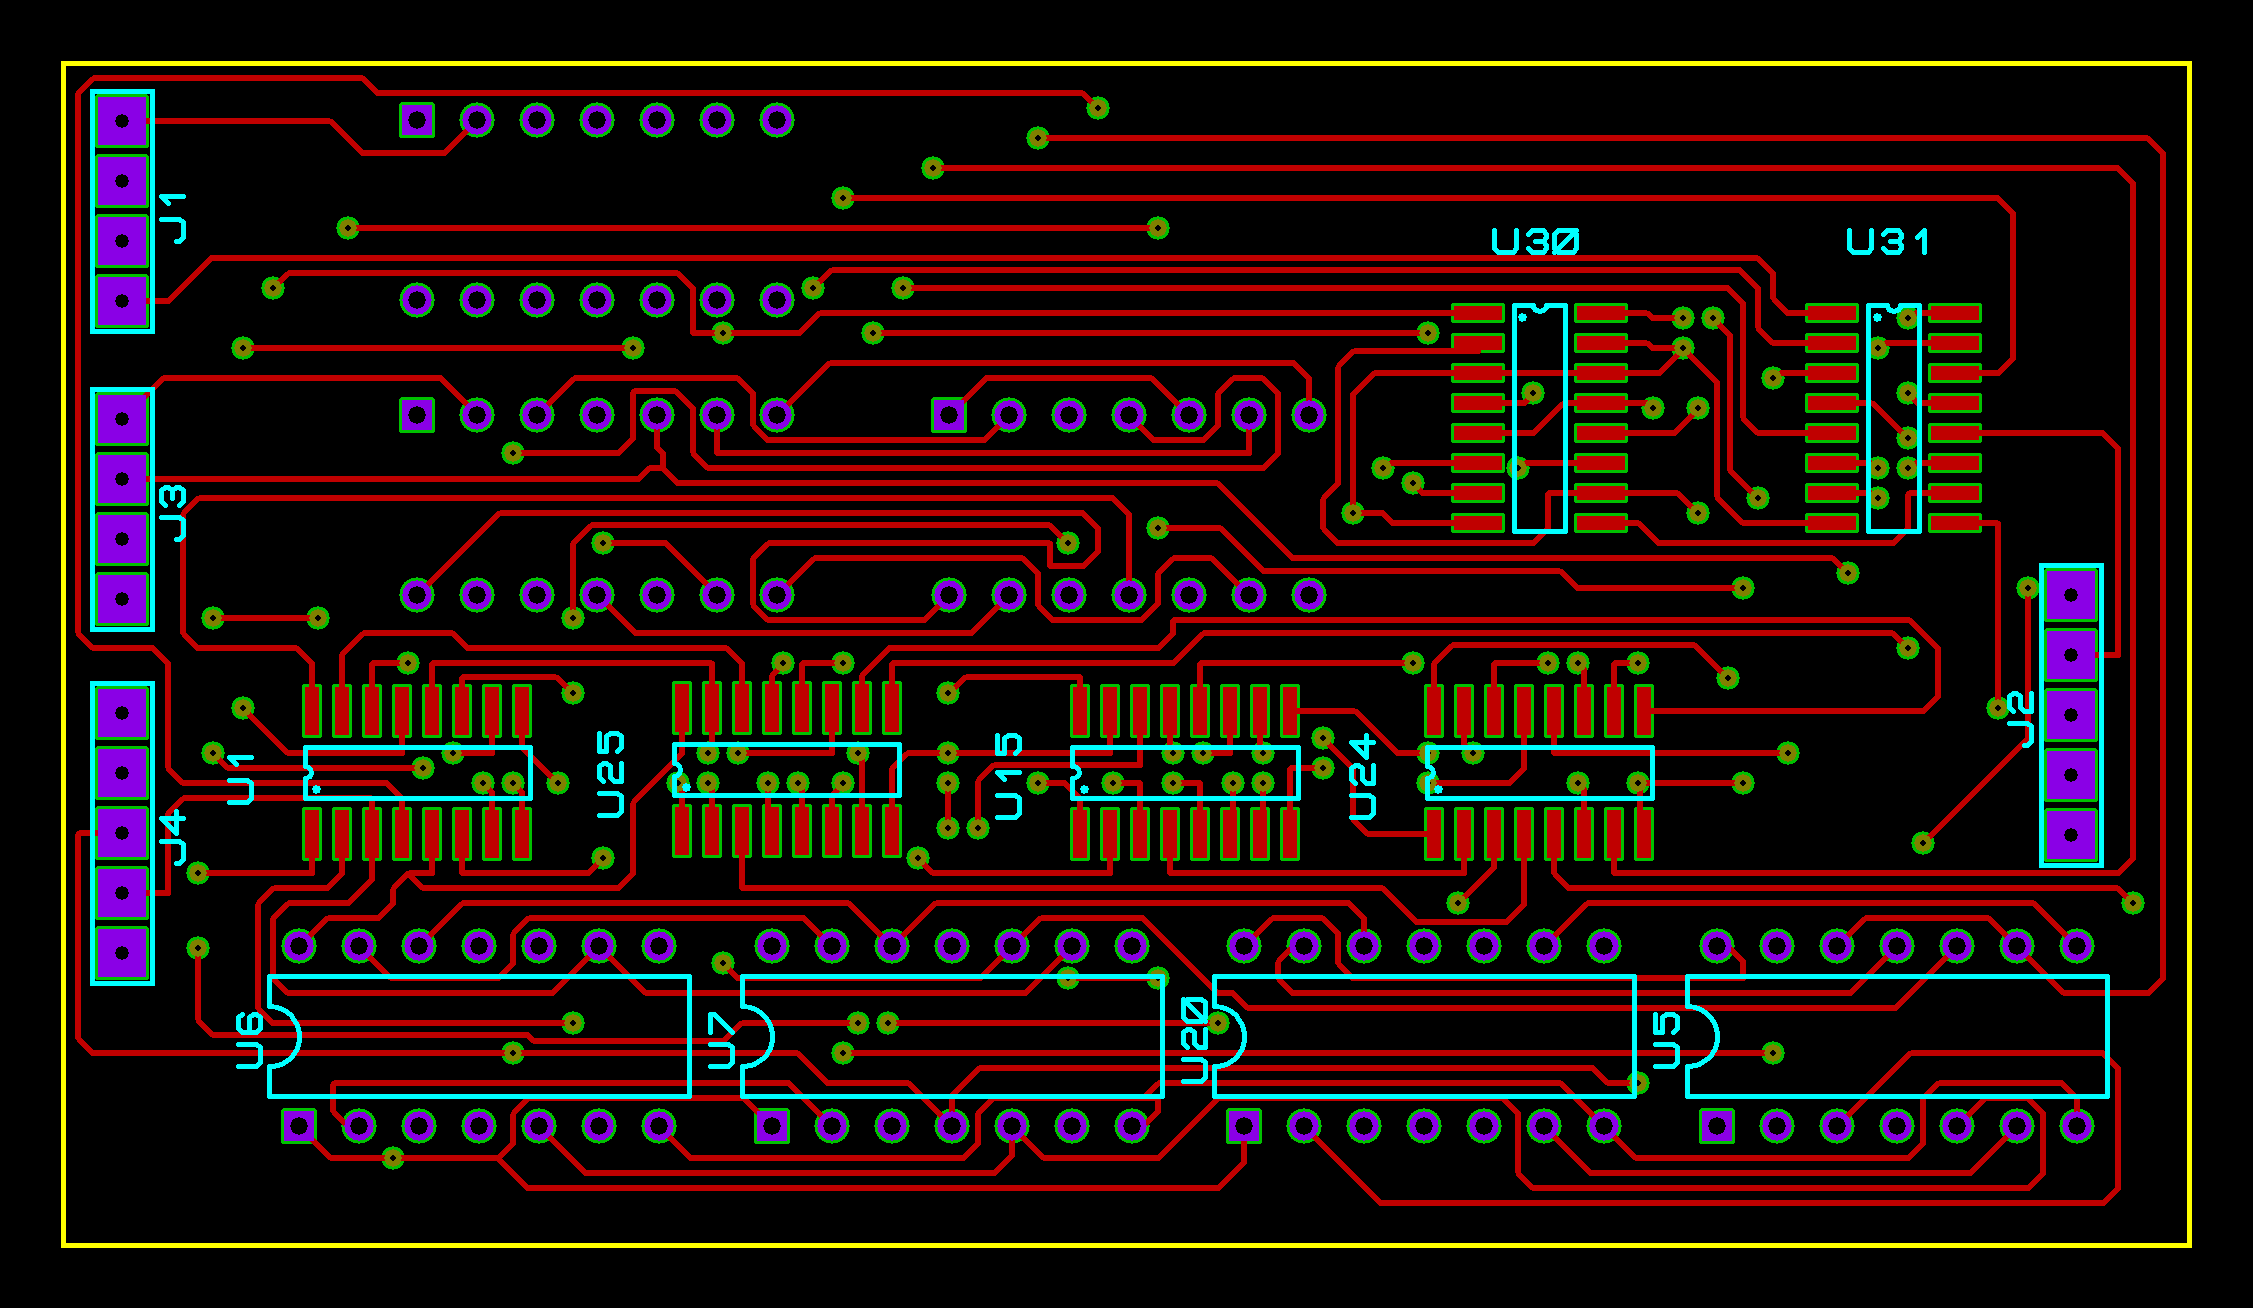
\includegraphics[width=\textwidth]{images/ALU-PCB-TOP.png}
    \caption{
    نمای بالای برد چاپی
    }
\end{figure}

